% This is the aspauthor.tex LaTeX file
% Copyright 2010, Astronomical Society of the Pacific Conference Series

\documentclass[11pt,twoside]{article}
\usepackage{asp2010}

\resetcounters
%\bibliographystyle{asp2010}
\markboth{K. Anderson, et al}{LOFAR and HDF5}
\begin{document}
\title{LOFAR and HDF5: Toward a New Radio Data Standard}
\author{Kenneth Anderson$^1$, A. Alexov$^1$, L. B\"{a}hren$^1$, J-M. Grie\ss meier$^2$,
M. Wise$^3$, G.A. Renting$^3$}
\affil{$^1$Astronomical Institute �Anton Pannekoek�, University of Amsterdam, Postbus 94249, 1090 GE Amsterdam, The Netherlands}
\affil{$^2$Laboratoire de Physique et Chimie de l'Environnement et de l'Espace
 (LPC2E),
3A Avenue de la Recherche, 45071 Orléans Cedex 2, France}
\affil{$^3$Netherlands Institute for Radio Astronomy (ASTRON), 
P.O. Box 2, 7990 AA Dwingeloo, The Netherlands}
\begin{abstract}
For decades now, scientific data volumes have experienced relentless,
exponential growth.  As a result, legacy astronomical data formats are
straining under a burden not conceived when these formats were first
introduced. With future astronomical projects ensuring this trend, ASTRON
and the LOFAR project are exploring the use of the Hierarchical Data Format,
version 5 (HDF5), for LOFAR radio data encapsulation. Most of LOFAR's
standard data products will be stored natively using the HDF5 format.
In addition, HDF5 analogues for traditional radio data structures such
as visibility data and spectral image cubes are also being developed.
The HDF5 libraries allow for the construction of potentially distributed,
entirely unbounded files.  The nature of the HDF5 format further provides
the ability to custom design a data encapsulation format.
The LOFAR project has designed several data formats that will accommodate
all LOFAR data products, examples of which are presented in this paper.
With proper development and support, it is hoped that these data formats
will be adopted by other astronomical projects as they, too,
attempt to grapple with a future filled with mountains of data.
\end{abstract}
\section{Introduction}
The commmencement of the operational phase of The LOw Frequency ARray (LOFAR) telescope holds
forth both great scientific potential and challenges to current and
legacy information technologies: volume and complexity of the data will
continue to push the envelope of commonly used data protocols.

Recognizing that this envelope is already strained, the LOFAR project has
embarked on an ambitious project to design and define a set of radio data
standard formats that are capable of encapsulating the full spectrum of,
not just LOFAR data products, but astronomical radio data in general.

It is with this ambition in mind that the LOFAR data formats group have
been developing these format specifications and associated software infrastructure,
an ongoing, two year effort to date. It was determined that HDF5 would be a
robust, viable data framework capable of handling the size, scope, diversity,
and parallel processing requirements of LOFAR data (\cite{BoF5_adassxx}).
This work certainly has potential use beyond the radio community.  New large scale
optical telescopes, such as the LSST, are also investigating the viability of
using HDF5. Furthermore, the 20 year history of HDF and its continuing use by NASA,
the NOAA, and other agencies, ensure broad use and and long term support.

In addition to the format descriptions themselves, the LOFAR project is
currently developing a set of software tools for creating and working with these
formats. The Data Access Library (DAL) in C++, along with an associated Python
interface (pyDAL), are designed to allow for the easy construction
and manipulation of these data formats. There are also a number of tools
already available to read and visualize HDF5 files, such as:
HDFView\footnote{HDFView: \url{http://www.hdfgroup.org/hdf-java-html/hdfview/}},
VisIt\footnote{VisIt: \url{https://wci.llnl.gov/codes/visit/}} + plugin,
PyTables\footnote{PyTables: \url{http://www.pytables.org/moin}},
h5py\footnote{h5py: \url{http://code.google.com/p/h5py/}},
MATLAB\footnote{MATLAB: \url{http://www.mathworks.com/products/matlab/}} and
IDL\footnote{IDL: \url{http://www.ittvis.com/ProductServices/IDL.aspx}}.
Additionally, the LOFAR project has started work on an HDF5 plugin for VisIt,
which is a visualization tool specializing in handling large datasets.
Initial communication has been opened with William Joye regarding
implementation of DS9 compatibility with LOFAR Sky Image Cubes.

\section{The LOFAR Radio Telescope}

LOFAR is nearing the end of construction in The Netherlands and throughout Europe.
There are currently 30 Dutch stations and 5 European stations actively observing
commissioning proposals.  Once LOFAR is completed, there will be 40 stations in
The Netherlands and at least 8 European/International stations.  LOFAR's
Low Band Antenna (LBA) functions in the range of 30-80 MHz and High Band Antenna
(HBA) is in the 120-240 MHz range;  the telescope bandwidth is 48MHz.
LOFAR can create 8 (possibly more) simultaneous beams, has a spectral resolution of
0.76 kHz (1 sec) and a time resolution of 5.1 nano-seconds.

The features of LOFAR that point to massive data volumes: 30,000 networked,
passive phased-array antenn\ae in The Netherlands; international baselines
to 1500 km; 6 Gb/s Data Rate, correlated by Blue Gene/P supercomputer, Groningen, NL;
Ability to form 8 (and possibly more) concurrent digital beams.

\section{LOFAR Data: Variety, Complexity, Volume}
Datasets produced by LOFAR observations will vary tremendously in size and complexity.
Images, Beam-formed (BF) data, Transient Buffer board time-series data
are expected to produce large files, with some observations potentially creating
files of several tens of terabytes (see Table ~\ref{tab:data-size}).

\begin{table}[hbt]
\begin{small}
  \centering
  \begin{tabular}{|ccccc|}
    \hline
    \sc Exposure & \sc Number of & \sc Number of & \sc File Size  & \sc File Size  \\
    \sc Time     & \sc Subbands  & \sc Stations  & \sc Known Mode & \sc Search Mode \\
    \hline \hline
     1 min & 248 & 20 & 11.2GB & 244GB \\
\hline
     10 min & 248 & 30 & 112GB & 3.3TB \\
\hline
     1 hr  & 248 & 10 & 672GB & 6.7TB \\
     1 hr  & 248 & 20 & 672GB & 13.4TB\\
     1 hr  & 248 & 30 & 672GB & 26.8TB \\
\hline
     2 hr  & 248 & 5 & 1.3TB & 6.7TB \\
\hline
     12 hr & 248 & 5 & 8.0TB & 40.3TB \\
     12 hr & 248 & 15 & 24.0TB & 120.1TB \\
    \hline
 \end{tabular}
  \caption{\scriptsize Sample, LOFAR BF dataset sizes for different observation times and
number of stations used.  The difference between Known and Search Mode is that data are
saved per station for searching, as apposed to combined when observing a known object
(to increase signal-to-noise and save disk space).}
  \label{tab:data-size}
\end{small}
\vskip -4mm
\end{table}

LOFAR's observational modes are capable of producing highly complex,
large volume datasets.  Legacy protocols fall short of being able to describe
or store these data. This looming predicament is especially
germane to the SKA pathfinder LOFAR project, wherein certain
operational modes will be capable of generating datasets comprising
hundreds of gigabytes to tens of terabytes.
Therefore, the LOFAR project has been driven to consider viable alternatives
to ``standard'' astronomical data formats, such as FITS and CASA Tables.
\footnote{For more detailed
discussion of LOFAR data rates, volume, complexity, and HDF5,
see~\cite{BoF5_adassxx},
\textit{Towards HDF5: Encapsulation of Large and/or Complex Astronomical Data,} BoF5, ADASS XX.}

\section{LOFAR Data Format Specifications}
A viable solution was needed for potentially massive LOFAR data products.
HDF5 provides a framework allowing users to essentially design their own
files to appropriately accommodate a known variety of datatypes (\cite{BoF5_adassxx}).
The LOFARproject has been engaged in developing and designing a complete set of
specifications for all LOFAR observational data. This has necessarily
required differing file designs for differing data, with a certain
structural parallelism maintained across all file designs.

These Interface Control Documents (ICD)\footnote{LOFAR ICDs are publicly available:
\url{http://usg.lofar.org/wiki/doku.php?id=documents:lofar_data_products}}
provide detailed descriptions of a range of  expected LOFAR Data Products,
including Radio Sky Images, Transient Time Series data, Beam-Formed data, Dynamic Spectra,
UV Visibility, Rotation Measure Synthesis, Near-field Imaging. By way of example, structures
of a LOFAR Radio Sky Image and a Dynamic Spectra file are outlined in
Figures ~\ref{fig:skyimDiag} and ~\ref{fig:dynspecDiag}.

\begin{figure}[htbp]
  \centering
  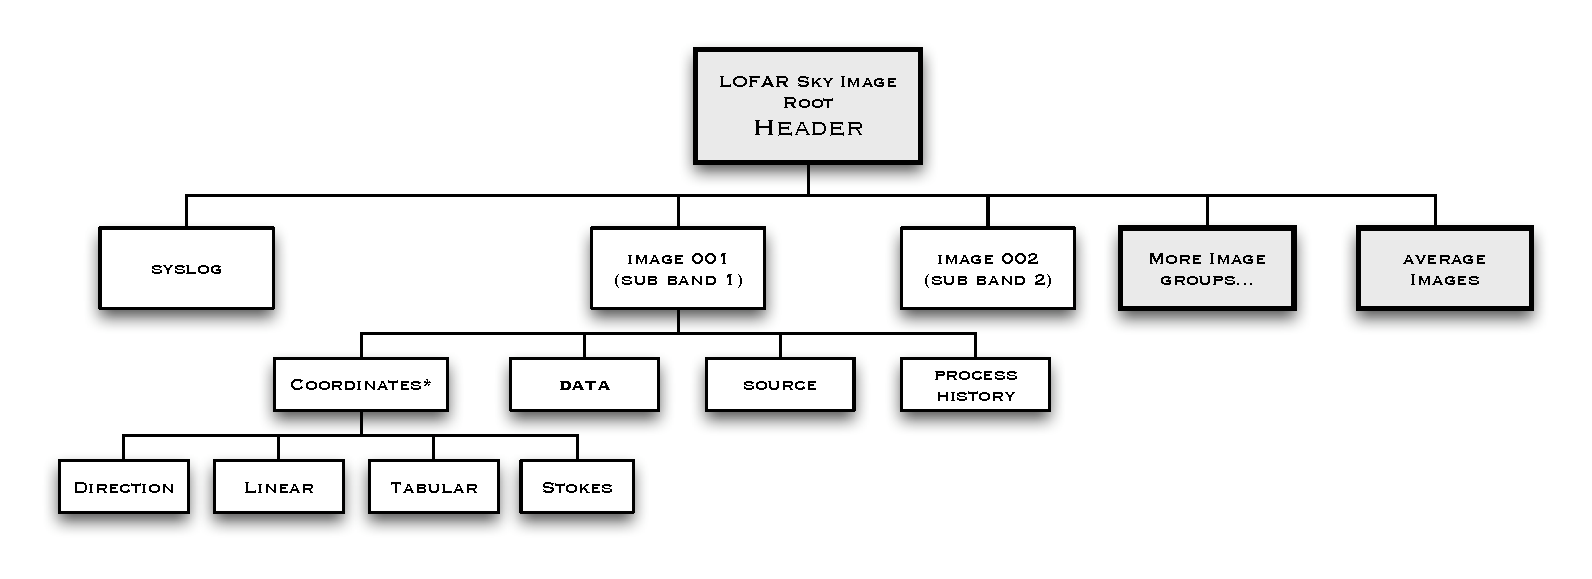
\includegraphics[scale=0.37]{SkyImDiag3_1.eps}
  \caption{LOFAR Radio Sky Image Data Structure}
  \label{fig:skyimDiag}
\vskip -4mm
\end{figure}

\begin{figure}[htbp]
 \centering
  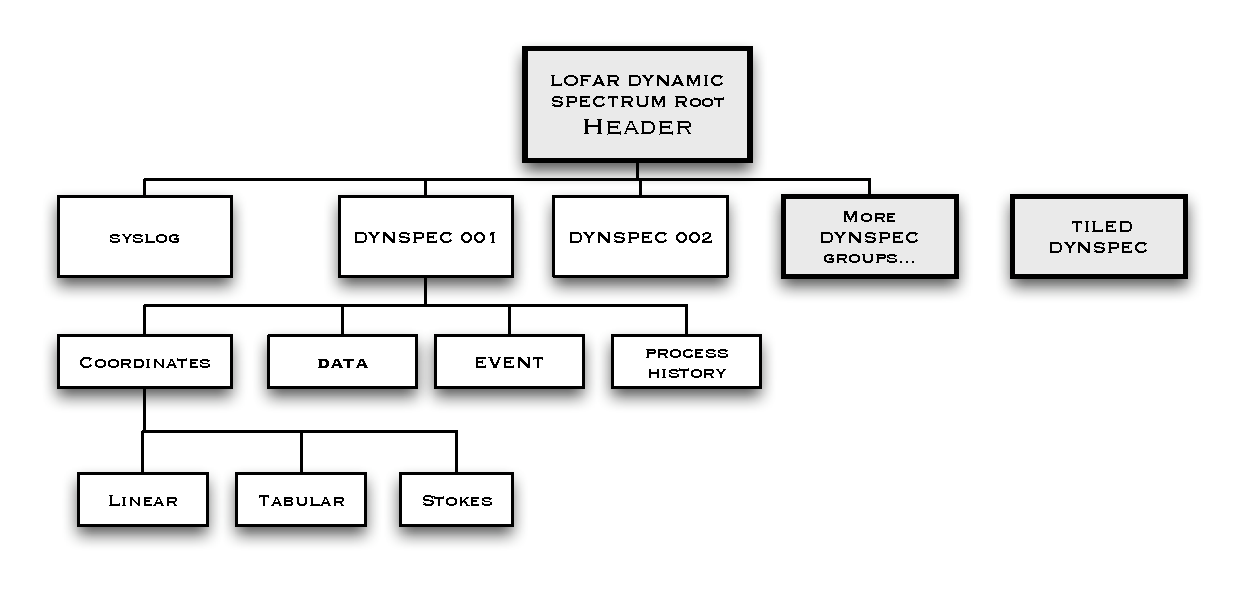
\includegraphics[scale=0.42]{DynSpec.eps}
   \caption{LOFAR Dynamic Spectra Data Structure}
   \label{fig:dynspecDiag}
 \vskip -4mm
\end{figure}

The LOFAR ICD team has also produced a document describing the coordinate
system for the file structure;  these coordinates are closely related to
the WCS for FITS.  It is not the intension of the project to redo decades
of WCS work which is already in place, but to map the LOFAR coordinates to
standard WCS.

\section{Summary and Future Considerations}

In order that adoption of LOFAR data formats prove useful in the real
world, the LOFAR project is committing resources to help develop the next
generation of astronomical tools for LOFAR data. A major effort of the
LOFAR project has been the development of the Data Access Library (DAL), which
ultimately will provide interfaces through FITS, the CASA/AIPS++ Measurement Sets
and HDF5. All LOFAR products will be accessible through DAL tools, which are part of the
LOFAR User Software (LUS)\footnote{LOFAR User Software Repository:
\url{http://usg.lofar.org/wiki/doku.php?id=development:getting_started}} repository.

The LOFAR project has set up a moderated majordomo email list, called 
\\ \textbf{nextgen-astrodata@astron.nl}.  Interested parties are encouraged to sign up via 
\\ \textbf{majordomo@astron.nl} with 
``\textbf{subscribe nextgen-astrodata}'' as the only text in the body of the message.
Ultimately we would like to see these formats grow into a true set of standards
for radio data that can meet the demands of the next generation of radio
observatories. Such standards are sorely lacking in the radio community at
present and are clearly needed as radio astronomy moves into the SKA epoch.

\acknowledgements The author would like to thank colleagues of the ICD development
group, ASTRON, the \textit{Sterrunkundig Instituut Anton Pannekoek},
the HDF Group, and the ADASS XX organizers for what proved to be an
excellent conference!

\bibliographystyle{asp2010}
\bibliography{P047}

\end{document}
